\documentclass[11pt]{article}
\usepackage[margin=1in]{geometry}
\usepackage{amsmath,amssymb,amsthm}
\usepackage{graphicx}
\usepackage{booktabs}
\usepackage{array}
\usepackage{xcolor}
\usepackage{algorithm}
\usepackage{algpseudocode}
\usepackage{hyperref}
\usepackage{subcaption}
\usepackage[capitalise,noabbrev]{cleveref}

\theoremstyle{definition}
\newtheorem{definition}{Definition}
\theoremstyle{plain}
\newtheorem{proposition}{Proposition}
\newcommand{\Psiu}{\Psi_u}

\begin{document}

\setcounter{section}{2}

\section{FSDP Architecture}
\label{sec:fsdp}

Fully Sharded Data Parallel (FSDP) lets us train models that are too
large for one GPU~\cite{zhao2023fsdp}. In plain data parallelism, every
GPU keeps a full copy of the model. FSDP does not. It splits the
parameters, gradients, and optimizer states across all GPUs, so each GPU
keeps only a small piece. When a GPU needs a layer, it collects the
missing pieces from the other GPUs, runs the layer, and then throws the
borrowed pieces away. This way, no single GPU ever has to hold the whole
model at once.

\subsection{Notation and Definitions}
\label{sec:notation}

~\ref{tab:notation} lists the symbols we use in this section.

\begin{table}[ht]
  \centering

  \begin{tabular}{lc}
    \toprule
    Symbol & Meaning \\
    \midrule
    $N$          & Number of GPUs  \\
    $\Psi$       & Total number of model parameters \\
    $\Psiu$      & Number of parameters in one FSDP unit \\
    $U$          & Number of FSDP units in the model \\
    $W$          & Parameters of one unit (flattened) \\
    $W_i$        & The $i$-th shard of $W$, owned by rank $i$ \\
    $g^{(i)}$    & Local gradient computed on GPU $i$ \\
    $g_i$        & The $i$-th shard of the averaged gradient $g$ \\
    $K$          & Optimizer-state bytes per parameter \\
    \bottomrule

  \end{tabular}

  \caption{Notation used in this section.}
  \label{tab:notation}
\end{table}

\begin{definition}[Sharding]
  \label{def:sharding}
  Sharding splits a tensor into $N$ pieces that do not overlap.
  Rank $i$ owns and stores the $i$-th piece.
\end{definition}

\begin{definition}[FSDP unit]
  \label{def:unit}
  An FSDP unit is a group of layers that FSDP treats as one block. FSDP
  flattens, shards, gathers, and frees the parameters of a unit
  together.
\end{definition}

\begin{figure}[ht]
  \centering
  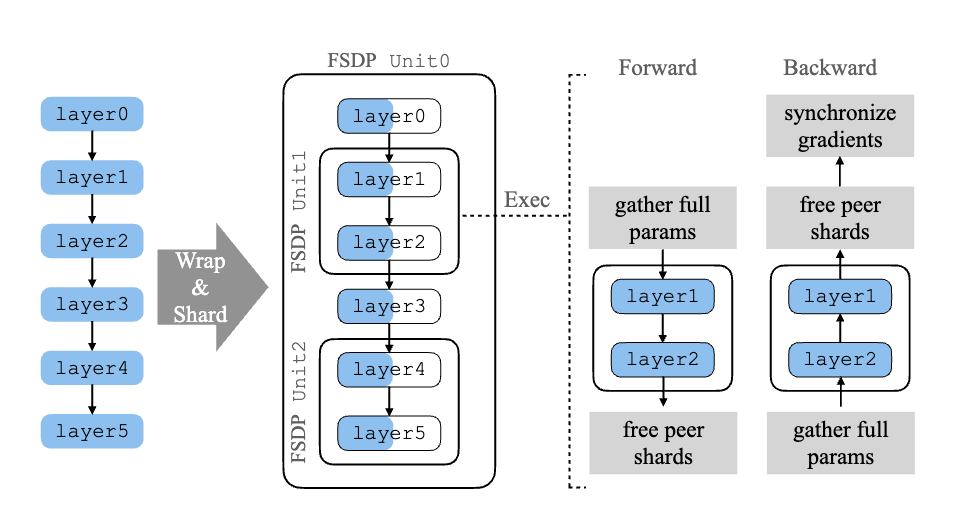
\includegraphics[width=0.8\linewidth]{wrap_shard.png}
  \caption{Wrapping a model into FSDP units. Layers~0 and~3 are not
    wrapped separately, so they belong to the outer unit, Unit~0.
  }
  \label{fig:wrap}
\end{figure}

~\ref{fig:wrap} shows how we split a six-layer model into FSDP units.
Unit~1 holds Layers~1 and~2. Unit~2 holds Layers~4 and~5. FSDP flattens
and shards each of these units on its own. Unit~0 wraps the whole
model. It picks up every layer that no inner unit claims, which here
means Layers~0 and~3.

The right side of the figure shows the life of one unit. In the forward
pass, the unit gathers its full parameters, runs its layers, and frees
the shards that other ranks own. In the backward pass, it gathers the
parameters again, computes gradients, frees the borrowed shards once
more, and syncs the gradients across ranks. At any moment, only the
active unit holds its full parameters. So the way we wrap the model
decides the peak memory. Smaller units mean less memory at the peak.

\subsection{Model State and Sharding}
\label{sec:model-state}

\subsubsection{Components of Model State}
\label{sec:components}

The model state has three parts: parameters, gradients, and optimizer
states. The parameters are the weights we train. The gradients tell us
how to change those weights, and we compute them in the backward pass.
The optimizer states are extra values that the optimizer keeps between
steps.

Take Adam with mixed-precision training as an example. Here the
optimizer keeps an fp32 copy of the weights, because fp16 alone loses
too much precision during updates. It also keeps the first and second
moment of the gradients, again in fp32. Together, these three values
take $K$ bytes per parameter~\cite{rajbhandari2020zero}.

\subsubsection{Replication in DDP versus Sharding in FSDP}
\label{sec:ddp-vs-fsdp-layout}

In Distributed Data Parallel (DDP), every GPU keeps a full copy of all
$\Psi$ parameters. Each GPU also keeps a full copy of the gradients and
the optimizer states. All $N$ GPUs store the same data. This wastes a
lot of memory, and large models quickly run out of room.

FSDP removes this waste. It takes the flattened parameters $W$ of each
unit and splits them into $N$ shards. Rank $i$ stores and updates only
its own shard $W_i$.

FSDP shards the gradients and the optimizer states in the same way.
Rank $i$ keeps only the gradient shard $g_i$ and the optimizer state for
the parameters in $W_i$. ~\ref{fig:ddp-fsdp-layout} compares the two
layouts. In DDP each GPU holds everything. In FSDP each GPU holds one
$N$-th of everything. This is why FSDP can train models that DDP cannot
fit.

\vspace{2\baselineskip}
\begin{figure}[ht]
  \centering
  \begin{subfigure}{0.45\linewidth}
    \centering
    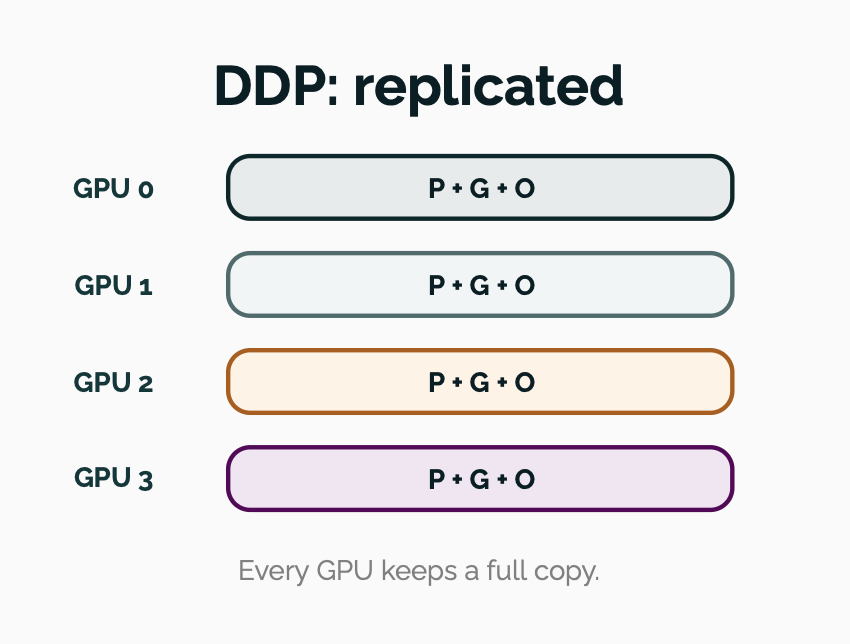
\includegraphics[width=\linewidth]{ddp.png}
    \caption{DDP memory layout.}
  \end{subfigure}%
  \hfill
  \begin{subfigure}{0.45\linewidth}
    \centering
    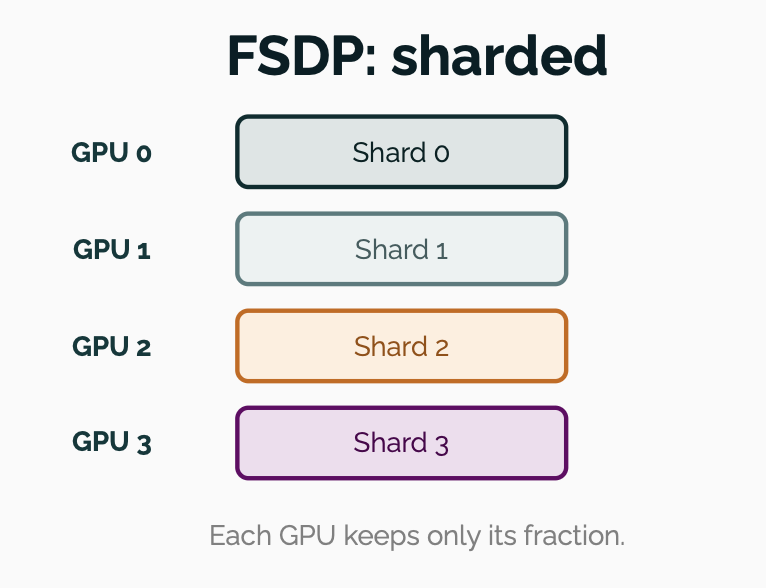
\includegraphics[width=\linewidth]{fsdp.png}
    \caption{FSDP memory layout.}
  \end{subfigure}

  \caption{Model-state memory layout under DDP (every GPU holds a full
  replica) and FSDP (every GPU holds one shard).}
  \label{fig:ddp-fsdp-layout}
\end{figure}

\subsubsection{Flattening and Padding}
\label{sec:flatten}

A layer usually has several tensors, such as a weight matrix and a bias
vector. Sharding each tensor one by one would be slow and messy. So FSDP
first joins all parameters of a unit into one long 1-D tensor. We call
this tensor the \texttt{FlatParameter}.

The length of the \texttt{FlatParameter} is $\Psiu$. This number may
not divide evenly by $N$. When it does not, FSDP adds a few zeros at the
end (padding) until the length is a multiple of $N$. Then it cuts the
tensor into $N$ equal shards. Each shard has the size given by
~\ref{eq:shard-size}.

\begin{equation}
  \text{shard size} = \left\lceil \frac{\Psiu}{N} \right\rceil
  \label{eq:shard-size}
\end{equation}

~\ref{fig:flatparam} shows an example with 16 GPUs. The unit has a
$3 \times 4$ weight (12 values) and a bias with 3 values, so
$\Psiu = 15$. FSDP joins them into one tensor of length 15 and adds one
padding value to reach 16. Each GPU then gets exactly one value. Ranks
0 to 14 hold real parameters, and rank 15 holds only the padding.

\begin{figure}[ht]
  \centering
  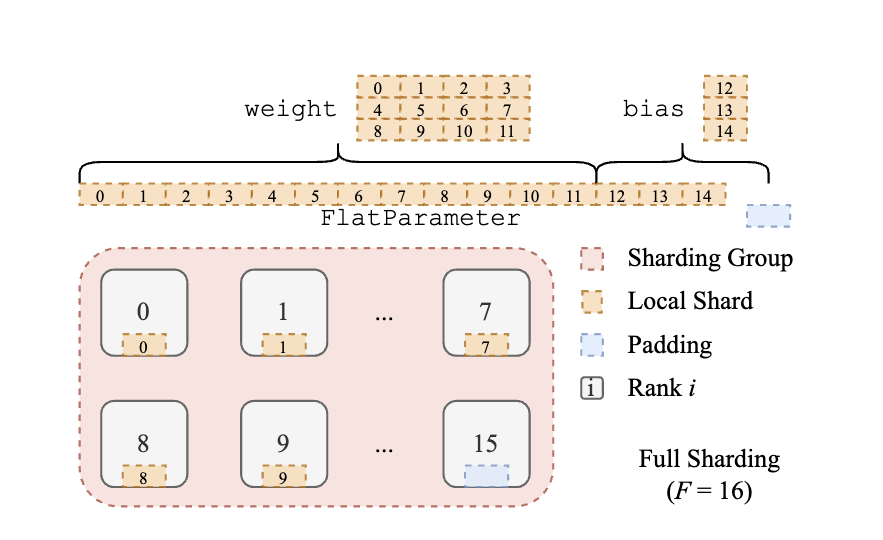
\includegraphics[width=0.75\linewidth]{flat-parameters.png}
  \caption{\texttt{FlatParameter} sharding across 16 GPUs. The weight
    and bias are joined into one 1-D tensor, padded to length 16, and
    split so that each rank owns one element. The symbol $F$ in the
  figure is $N$ in our notation.}
  \label{fig:flatparam}
\end{figure}

\subsection{Collective Communication Primitives}
\label{sec:collectives}

FSDP moves data between GPUs with two collective operations:
All-Gather and Reduce-Scatter. In a collective, all $N$ ranks take part
at the same time.

\subsubsection{All-Gather}
\label{sec:allgather}

All-Gather turns shards into a full tensor. Each rank starts with its
own shard $W_i$. Each rank sends its shard to every other rank. At the
end, every rank holds the full tensor $W$.

~\ref{fig:allgather} shows this for four GPUs. Before the call, each
GPU stores only $|W|/N$ values. This shard is persistent: the GPU keeps
it for the whole training run. After the call, each GPU holds all $|W|$
values. This full copy is transient: the GPU frees it as soon as it
finishes using it. Each rank already has its own shard, so it only
receives the other $N-1$ shards. ~\ref{eq:allgather} gives the amount
of data each rank receives.

\begin{equation}
  V_{\text{AG}} = \frac{N-1}{N}\,|W|
  \label{eq:allgather}
\end{equation}

\vspace{1\baselineskip}

\begin{figure}[ht]
  \centering
  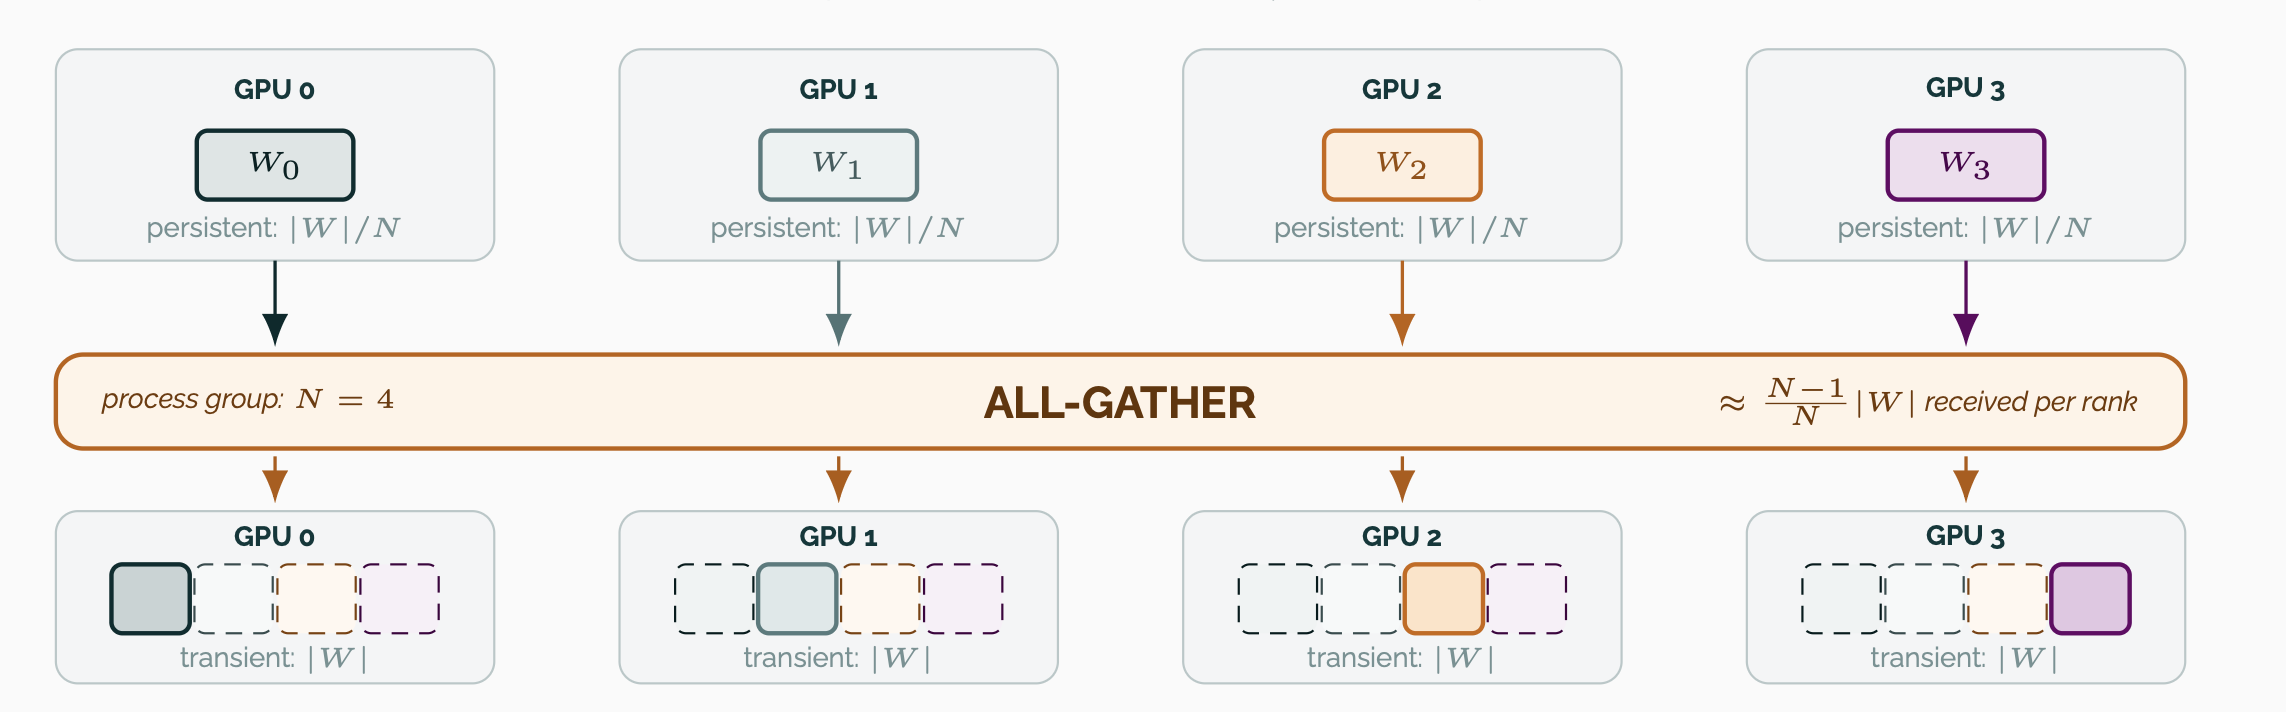
\includegraphics[width=\linewidth]{all-gather.png}
  \caption{All-Gather on four GPUs. Each GPU starts with one persistent
  shard $W_i$ and ends with a transient copy of the full tensor $W$.}
  \label{fig:allgather}
\end{figure}

\subsubsection{Reduce-Scatter}
\label{sec:reducescatter}

Reduce-Scatter works in the other direction. Each rank starts with a
full tensor $G$ of the same size. The ranks add their tensors together
element by element. But no rank ends up with the full sum. Instead, rank
$i$ gets only the $i$-th shard of the sum.

Reduce-Scatter is one single collective. It is not a Reduce call
followed by a Scatter call. No rank ever builds the full sum, so no rank
needs the extra memory for it. Each rank sends and receives about the
same amount of data as in All-Gather:

\begin{equation}
  V_{\text{RS}} = \frac{N-1}{N}\,|G|
  \label{eq:reducescatter}
\end{equation}

\subsubsection{Relation to All-Reduce}
\label{sec:allreduce}

DDP syncs its gradients with All-Reduce. All-Reduce adds the tensors
from all ranks and gives the full sum to every rank. We can split
All-Reduce into two steps. First, a Reduce-Scatter gives each rank one
shard of the sum. Then, an All-Gather sends every shard to every rank.
So All-Reduce equals Reduce-Scatter plus All-Gather, and it moves about
twice as much data as either one alone.

FSDP uses these two halves on their own. It uses All-Gather to rebuild
parameters and Reduce-Scatter to sync gradients. Note that a plain
All-Reduce gives a sum. FSDP wants the average gradient, so it also
divides the result by $N$.

\subsection{Forward Pass}
\label{sec:forward}

\subsubsection{Why a Layer Needs Full Parameters}
\label{sec:why-full}

Think of a linear layer that computes $y = Wx$. Every output value
depends on a full row of $W$. Rank $i$ holds only the shard $W_i$, which
is a small slice of the flattened tensor. With only $W_i$, rank $i$
cannot compute $y$. It needs all of $W$. So before a unit runs, every
rank must collect the full parameters of that unit.

\subsubsection{Gather, Compute, Reshard}
\label{sec:gather-compute-reshard}

The forward pass handles one unit at a time in three steps:
\begin{enumerate}
  \item \textbf{Gather.} The ranks call All-Gather on their shards.
    Every rank now holds the full $W$ of the unit.
  \item \textbf{Compute.} Each rank runs the unit on its own
    mini-batch.
  \item \textbf{Reshard.} Each rank frees the parts of $W$ that it does
    not own. It keeps only $W_i$.
\end{enumerate}
The full parameters live only for a short time, while the unit runs.
The shard $W_i$ stays in memory for the whole training run. Then the
next unit repeats the same steps.

\subsection{Backward Pass and Gradient Synchronization}
\label{sec:backward}

\subsubsection{Re-gathering Parameters}
\label{sec:regather}

The backward pass also needs the full parameters, because computing the
gradient of a layer uses its weights. But FSDP freed those weights right
after the forward pass. So each unit calls All-Gather again before its
backward step. The backward pass visits the units in reverse order, from
the last unit to the first. After the backward step, each rank frees the
borrowed parameters again.

\subsubsection{Local Gradients}
\label{sec:local-grads}

Each GPU trains on a different mini-batch. So when GPU $i$ runs the
backward pass, it gets its own local gradient $g^{(i)}$. These local
gradients differ from GPU to GPU. If each GPU used its own gradient to
update the model, the shards would drift apart. So the GPUs must first
agree on one gradient.

\subsubsection{Synchronization by Reduce-Scatter}
\label{sec:grad-sync}

FSDP uses the average of all local gradients as the true gradient.
~\ref{eq:grad-avg} defines it. Rank $i$ does not need the whole average.
It only updates $W_i$, so it only needs the matching shard $g_i$. A
Reduce-Scatter gives each rank exactly that shard. After the call, FSDP
divides by $N$ to turn the sum into an average.

\begin{equation}
  g = \frac{1}{N} \sum_{i=1}^{N} g^{(i)},
  \qquad \text{rank } i \text{ keeps only } g_i
  \label{eq:grad-avg}
\end{equation}

~\ref{tab:grad-example} and ~\ref{fig:reducescatter} show a small
example with four GPUs. Each GPU computes a local gradient with four
values. The average of the four vectors is $[1.5,\ 1.5,\ 2.0,\ 1.5]$.
GPU~$i$ keeps only the $i$-th value of this average. For example, GPU~2
keeps $(0 + 4 + 1 + 3)/4 = 2.0$.

\begin{table}[ht]
  \centering
  \caption{Worked four-GPU example of gradient synchronization by
  Reduce-Scatter.}
  \label{tab:grad-example}
  \begin{tabular}{@{}lcc@{}}
    \toprule
    GPU & Local gradient $g^{(i)}$ & Shard kept $g_i$ \\
    \midrule
    0 & $[2,\ 1,\ 0,\ 3]$ & $1.5$ \\
    1 & $[1,\ 2,\ 4,\ 0]$ & $1.5$ \\
    2 & $[3,\ 1,\ 1,\ 2]$ & $2.0$ \\
    3 & $[0,\ 2,\ 3,\ 1]$ & $1.5$ \\
    \midrule
    \multicolumn{3}{@{}l}{Averaged gradient $g = [1.5,\ 1.5,\ 2.0,\ 1.5]$} \\
    \bottomrule
  \end{tabular}
\end{table}

\begin{figure}[ht]
  \centering
  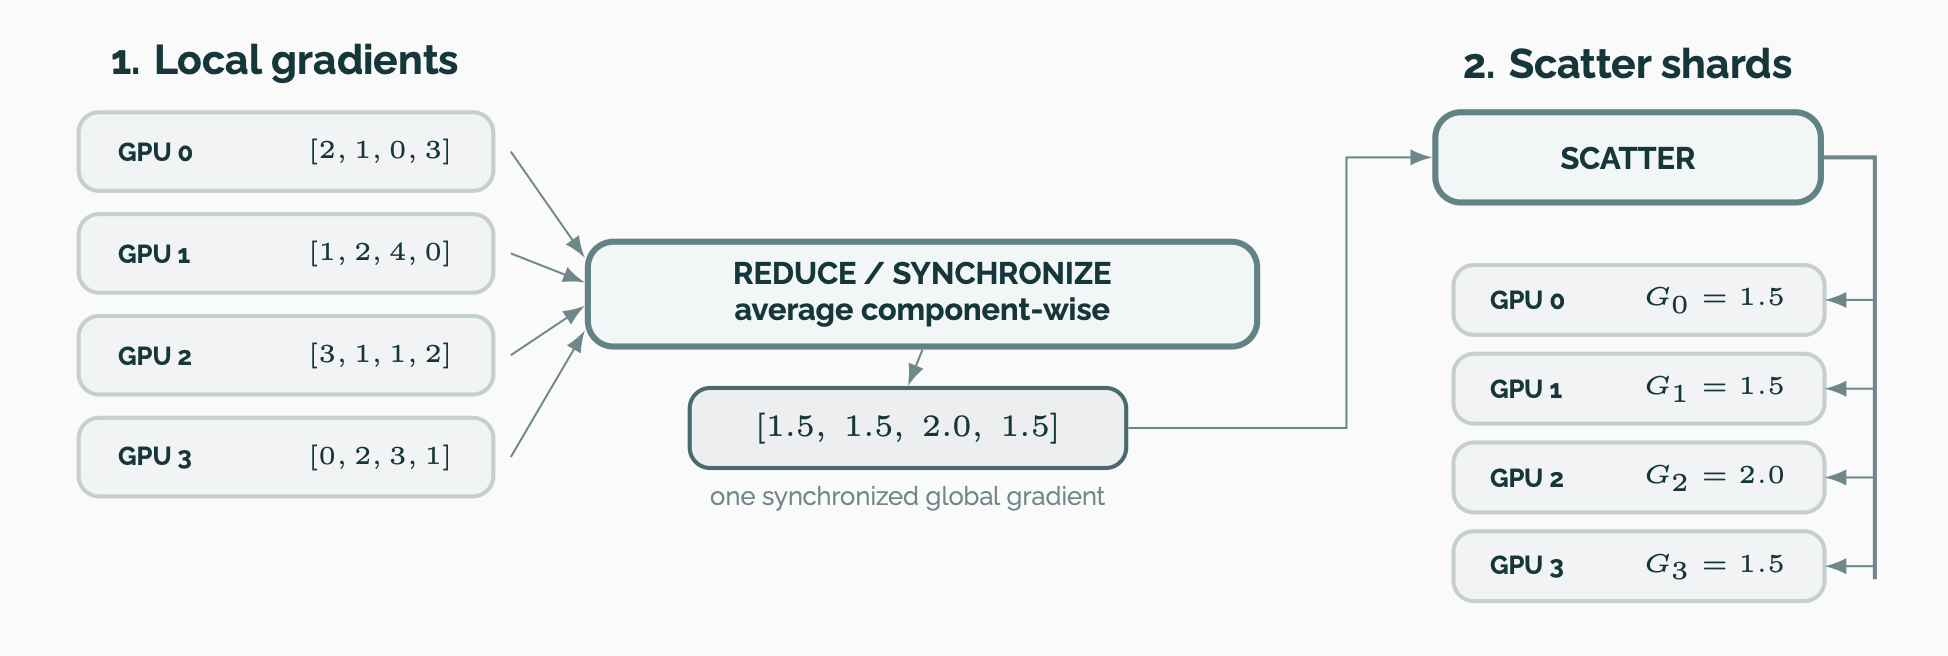
\includegraphics[width=0.9\linewidth]{reduce-scatter.png}
  \caption{Gradient synchronization on four GPUs. The local gradients
    are averaged element by element, and each GPU keeps one shard of the
  result. The symbol $G_i$ in the figure is $g_i$ in our notation.}
  \label{fig:reducescatter}
\end{figure}

\subsection{Optimizer Step}
\label{sec:optimizer}

After the backward pass, rank $i$ holds three things for its shard: the
parameters $W_i$, the averaged gradient $g_i$, and the optimizer state
for $W_i$. That is all it needs to run the optimizer. So each rank
updates its own shard on its own. The ranks do not talk to each other in
this step. Together, the $N$ updated shards form the full updated
model, which is the same model that DDP would produce.

\subsection{The Complete Training Iteration}
\label{sec:iteration}

~\ref{alg:fsdp} puts all the steps together. It shows one FSDP training
iteration on rank $i$:

\begin{algorithm}[ht]
  \caption{One FSDP training iteration on rank $i$}
  \label{alg:fsdp}
  \begin{algorithmic}[1]
    \Require Parameter shards $W^{(u)}_i$ and optimizer-state shards for
    every unit $u = 1,\dots,U$; local mini-batch $x^{(i)}$
    \Statex \textit{// Forward pass}
    \For{$u = 1$ \textbf{to} $U$}
    \State $W^{(u)} \gets \textsc{AllGather}\big(W^{(u)}_i\big)$
    \State Compute forward of unit $u$ with $W^{(u)}$
    \State Free all of $W^{(u)}$ except $W^{(u)}_i$ \Comment{reshard}
    \EndFor
    \State Compute loss $\mathcal{L}$
    \Statex \textit{// Backward pass}
    \For{$u = U$ \textbf{down to} $1$}
    \State $W^{(u)} \gets \textsc{AllGather}\big(W^{(u)}_i\big)$
    \State Compute local gradient $g^{(i),u}$ of unit $u$
    \State Free all of $W^{(u)}$ except $W^{(u)}_i$
    \State $g^{(u)}_i \gets \textsc{ReduceScatter}\big(g^{(i),u}\big) / N$
    \State Free $g^{(i),u}$
    \EndFor
    \Statex \textit{// Optimizer step (local, no communication)}
    \For{$u = 1$ \textbf{to} $U$}
    \State Update $W^{(u)}_i$ using $g^{(u)}_i$ and its optimizer-state shard
    \EndFor
  \end{algorithmic}
\end{algorithm}

\newpage
\begin{thebibliography}{9}
  \bibitem{rajbhandari2020zero}
  S.~Rajbhandari, J.~Rasley, O.~Ruwase, and Y.~He.
  \newblock ZeRO: Memory optimizations toward training trillion parameter
  models.
  \newblock In \emph{SC20: International Conference for High Performance
  Computing, Networking, Storage and Analysis}, 2020.

  \bibitem{zhao2023fsdp}
  Y.~Zhao, A.~Gu, R.~Varma, L.~Luo, C.-C. Huang, M.~Xu, L.~Wright,
  H.~Shojanazeri, M.~Ott, S.~Shleifer, A.~Desmaison, C.~Balioglu,
  P.~Damania, B.~Nguyen, G.~Chauhan, Y.~Hao, A.~Mathews, and S.~Li.
  \newblock PyTorch FSDP: Experiences on scaling fully sharded data
  parallel.
  \newblock \emph{Proceedings of the VLDB Endowment}, 16(12):3848--3860,
  2023.
\end{thebibliography}

\end{document}
